\section{Implementation}
\label{sec:num:implementation}
All our implementations use the Julia language \cite{bezanson-edelman-karpinski-shah-2017}.
We utilized our local workstation to generate the results on the CPU, which is equipped with an AMD EPYC 7443 processor (3.2GHz) with 24 processors.
For the GPU results, we used an NVIDIA A100 GPU (with CUDA 12.3) on the Polaris testbed at Argonne National Laboratory
\footnote{\url{https://www.alcf.anl.gov/polaris}}.
\add{Julia uses Just-in-Time (JIT) compilation to compile the code at runtime.
  The wall-time reported in the benchmarks does not include the compilation time.
}


\paragraph{IPM solver.}
We have implemented the two condensed-space methods in our nonlinear IPM solver MadNLP~\cite{shin2021graph}.
This implementation utilizes the {\tt AbstractKKTSystem} abstraction
in MadNLP to represent various KKT linear systems.
MadNLP can execute most of the IPM algorithm on the GPU.
In particular, all array manipulations are performed by GPU kernels, avoiding data transfers to host memory.
We refer to \cite{shin2023accelerating} for a detailed description of the GPU implementation in MadNLP.


\paragraph{Evaluation of the nonlinear models.}
For fast evaluation of the derivatives on the GPU,
we use ExaModels~\cite{shin2023accelerating}.
ExaModels harnesses the sparsity structure and provides custom derivative
kernels for repetitive algebraic subexpressions in constraints and
objective functions, enabling parallel first and second-order derivative computations on the GPU~\cite{bischof1991exploiting,enzyme2021}.
This approach caters to the SIMD architecture of the GPU by assigning multiple threads
to compute derivatives for different expression values.
ExaModels is highly efficient at evaluating problem derivatives, offering speedups often greater than 100 compared
to standard tools such as AMPL or JuMP (see Figure~\ref{fig:examodels}). As a
result, the time spent evaluating the model becomes
negligible compared to the time spent in the linear solver.
ExaModels compiles the derivative evaluation kernels specifically for a
given problem, whereas JuMP and AMPL rely on a precompiled interpreter to evaluate the model's derivatives.
However, ExaModels requires compilation time to create the derivative
evaluation kernels, which can become substantial for problems involving a
large number of heterogeneous constraints.
Throughout this paper, reported timings exclude compilation time.

\begin{figure}[!ht]
  \centering
  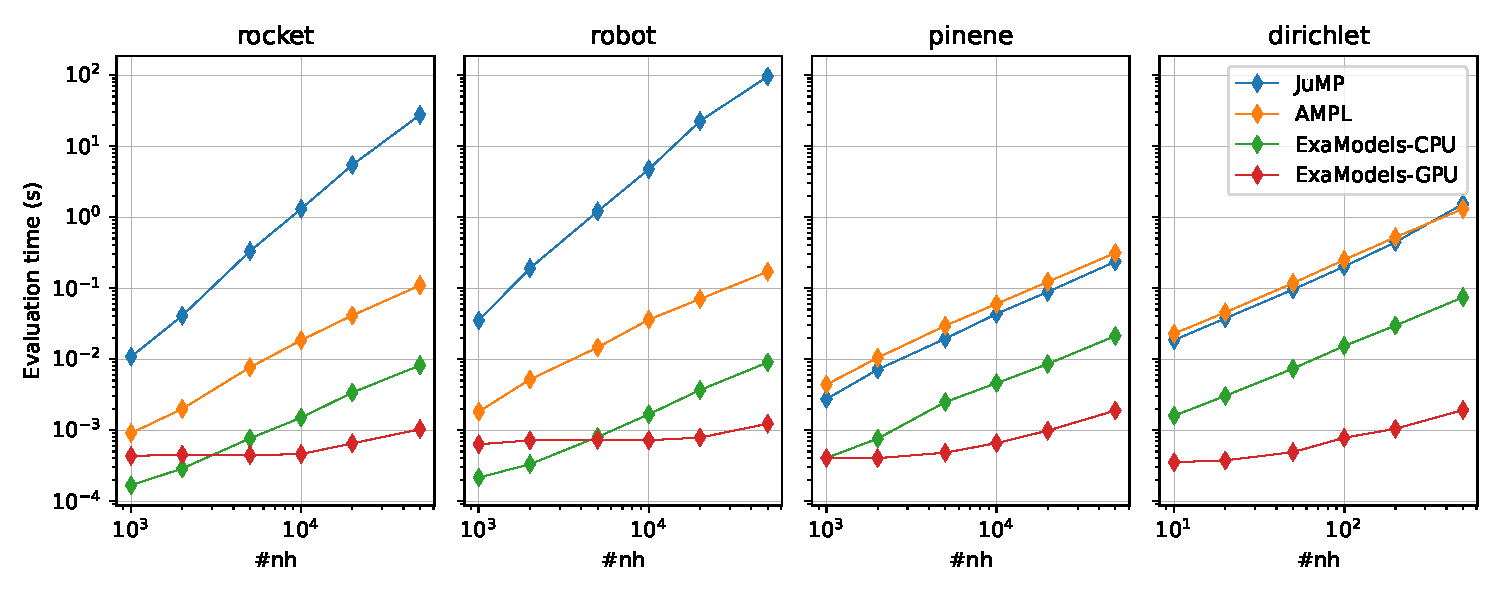
\includegraphics[width=.9\textwidth]{figures/benchmark_autodiff.pdf}
  \caption{Time spent evaluating problem derivatives (gradient, Jacobian, Hessian)
      as the problem dimension {\tt nh} increases. This benchmark compares four
  instances from the COPS benchmark~\cite{dolan2002benchmarking}: {\tt rocket}, {\tt robot}, {\tt pinene}, and {\tt dirichlet}.}
  \label{fig:examodels}
\end{figure}

\paragraph{Linear solvers.}
The KKT systems assembled in MadNLP are solved using various sparse linear
solvers, selected based on the KKT formulation (\eqref{eq:kkt:condensed},
\eqref{eq:kkt:augmented}, \eqref{eq:kkt:unreduced}) and the device (CPU, GPU).
We use the following solvers:
\begin{itemize}
  \item {\tt HSL MA27}: Implements the multifrontal \lblt factorization on the CPU~\cite{duff1983multifrontal}.
    \add{HSL MA27 supports single-threading only.}
  \item {\tt HSL MA57}: Implements the multifrontal \lblt factorization on the CPU~\cite{duff1983multifrontal},
    using multithreaded BLAS kernels in the elimination algorithm.
  \item {\tt HSL MA86}: Implements a fine-grained multicore parallel supernodal \lblt factorization on the CPU.
  \item {\tt Panua Pardiso}: Implements shared-memory parallel supernodal Cholesky, \ldlt and \lblt factorizations on the CPU.
  \item {\tt CHOLMOD}: Implements Cholesky and \ldlt factorizations on the CPU % Sungho: Maybe LDLFactorizations.jl instead, once the results are updated.
    (using AMD ordering \cite{amestoy-david-duff-2004} by default).
    It factorizes the condensed matrices $K_\gamma$ and $K_\tau$ appearing
    in \eqref{eq:kkt:hykkt} and \eqref{eq:liftedkkt}, respectively.
    \add{CHOLMOD supports multithreading.}
  \item {\tt cuDSS}: Implements \llt, \ldlt and \lu decompositions on NVIDIA GPUs.
    We use \ldlt factorization to decompose the ill-conditioned condensed matrices $K_\gamma$ on the GPU,
    (here, we have observed that \ldlt is more robust than Cholesky factorization).
  \item {\tt Krylov.jl}: Contains the \CG method
    used in the Golub \& Greif strategy to solve \eqref{eq:kkt:schurcomplhykkt} on both CPU and GPU architectures.
    \add{In our experiments, Krylov.jl runs in serial on the CPU.}
\end{itemize}
CHOLMOD is included with Julia.
For HSL linear solvers, we use libHSL \cite{fowkes-lister-montoison-orban-2024} with the Julia interface HSL.jl \cite{montoison-orban-hsl-2021}.
HSL MA57 and CHOLMOD are both compiled with OpenBLAS, a multithreaded version of BLAS and LAPACK.
Krylov.jl~\cite{montoison2023krylov} provides a collection
of Krylov methods with a polymorphic implementation suitable for both
CPU and GPU architectures.


%%% Local Variables:
%%% mode: LaTeX
%%% TeX-master: "../main"
%%% End:
